\documentclass[a4paper]{article}
\usepackage{setspace}
\usepackage[T2A]{fontenc} %
\usepackage[utf8]{inputenc} % подключение русского языка
\usepackage[russian]{babel} %
\usepackage[12pt]{extsizes}
\usepackage{mathtools}
\usepackage{graphicx}
\usepackage{fancyhdr}
\usepackage{amssymb}
\usepackage{amsmath, amsfonts, amssymb, amsthm, mathtools}
\usepackage{tikz}

\usetikzlibrary{positioning}
\setstretch{1.3}

\newcommand{\mat}[1]{\begin{pmatrix} #1 \end{pmatrix}}
\renewcommand{\det}[1]{\begin{vmatrix} #1 \end{vmatrix}}
\renewcommand{\f}[2]{\frac{#1}{#2}}
\newcommand{\dspace}{\space\space}
\newcommand{\s}[2]{\sum\limits_{#1}^{#2}}
\newcommand{\mul}[2]{\prod_{#1}^{#2}}
\newcommand{\sq}[1]{\left[ {#1} \right]}
\newcommand{\gath}[1]{\left[ \begin{array}{@{}l@{}} #1 \end{array} \right.}
\newcommand{\case}[1]{\begin{cases} #1 \end{cases}}
\newcommand{\ts}{\text{\space}}
\newcommand{\lm}[1]{\underset{#1}{\lim}}
\newcommand{\suplm}[1]{\underset{#1}{\overline{\lim}}}
\newcommand{\inflm}[1]{\underset{#1}{\underline{\lim}}}

\renewcommand{\phi}{\varphi}
\newcommand{\lr}{\Leftrightarrow}
\renewcommand{\r}{\Rightarrow}
\newcommand{\rr}{\rightarrow}
\renewcommand{\geq}{\geqslant}
\renewcommand{\leq}{\leqslant}
\newcommand{\RR}{\mathbb{R}}
\newcommand{\CC}{\mathbb{C}}
\newcommand{\QQ}{\mathbb{Q}}
\newcommand{\ZZ}{\mathbb{Z}}
\newcommand{\VV}{\mathbb{V}}
\newcommand{\NN}{\mathbb{N}}
\newcommand{\OO}{\underline{O}}
\newcommand{\oo}{\overline{o}}


\DeclarePairedDelimiter\abs{\lvert}{\rvert} %
\makeatletter                               % \abs{}
\let\oldabs\abs                             %
\def\abs{\@ifstar{\oldabs}{\oldabs*}}       %

\begin{document}

\section*{Домашнее задание на 30.01 (Математический анализ)}
 {\large Емельянов Владимир, ПМИ гр №247}\\\\
\begin{enumerate}
    \item[\textbf{№1}]
    \begin{enumerate}
        \item[(a)]
        Начнем с преобразования угла:
        $$
        \cos(816^\circ) = \cos(2 \cdot 360^\circ + 96^\circ) = \cos(96^\circ) = \cos\left(\frac{8\pi}{15}\right)
        $$
        Оценим остаточный член:
        $$\abs{R_n\left(\f{8\pi}{15}\right)}=\abs{(cos(\f{8\pi}{15}))^{(n+1)}\f{(\f{8\pi}{15}-\f{\pi}{2})^{n+1}}{(n+1)!}} \leq \f{(\f{16\pi}{30}-\f{15\pi}{30})^{n+1}}{(n+1)!} = \f{(\f{\pi}{30})^{n+1}}{(n+1)!} \leq 10^{-4} $$
        $$n=1: \f{\pi^2}{1800} > 10^{-4}$$
        $$n=2: \f{\pi^3}{162000} > 10^{-4}$$
        $$n=3: \f{\pi^4}{19440000} < 10^{-4}$$
        Следовательно, 
        $$\cos(x) \approx f\left(\frac{\pi}{2}\right) + f'\left(\frac{\pi}{2}\right)(x - \frac{\pi}{2}) + \frac{f''\left(\frac{\pi}{2}\right)}{2!}(x - \frac{\pi}{2})^2 + \frac{f'''\left(\frac{\pi}{2}\right)}{3!}(x - \frac{\pi}{2})^3$$
        $$
        \cos(x) \approx 0 - 1 \cdot \left(x - \frac{\pi}{2}\right) + 0 \cdot \frac{(x - \frac{\pi}{2})^2}{2!} + 1 \cdot \frac{(x - \frac{\pi}{2})^3}{3!}
        $$
        $$
        \cos(x) \approx -\left(x - \frac{\pi}{2}\right) + \frac{(x - \frac{\pi}{2})^3}{6}
        $$
        $$
        \cos{\frac{8\pi}{15}} \approx \frac{-5400\pi + \pi^3}{162000}
        $$
        \textbf{Ответ: }$\frac{-5400\pi + \pi^3}{162000}$\\

        \item[(b)]$\sqrt[4]{83}$

        Рассмотрим функцию:
        $$f(x) = (1 + x)^{\f{1}{4}}$$
        Оценим остаточный член:
        $$R_n(82, 80) = \f{f^{(n+1)}(c)}{(n+1)!}(82-80)^{n+1} \leq 2^{n+1}\f{\f{1}{4}(1 + 82)^{-\f{3}{4}}}{(n+1)!} =2^{n-1}\f{83^{-\f{3}{4}}}{(n+1)!} < 10^{-4}$$
        $$n=6: 2^{1-1}\f{83^{-\f{3}{4}}}{(1+1)!} > 10^{-4}$$
        $$n=7: 2^{2-1}\f{83^{-\f{3}{4}}}{(2+1)!} < 10^{-4}$$
        Следовательно,
        $$
        f(x) \approx 3 + \frac{1}{108}(x - 80) - \frac{3}{233280}(x - 80)^2 + \frac{21}{3840}(x - 80)^3 -$$$$- \frac{231}{61440}(x - 80)^4 + \frac{3003}{122880}(x - 80)^5 - \frac{5005}{2949120}(x - 80)^6 + \frac{6435}{82575360}(x - 80)^7
        $$
        $$f(82) \approx \f{70911455449}{23782864896}$$
        \textbf{Ответ:}$\f{70911455449}{23782864896}$

    \end{enumerate}

    \item[\textbf{№2}]
    \begin{enumerate}
        \item[(a)]Докажем, что:
        $$0 < n! \cdot (e - \s{k=0}{n}\f{1}{k!}) < 1$$
        Разложим $e^x$ в нуле:
        $$e^x = \s{k=0}{n}\f{x^k}{k!} + \f{c^{n+1}}{(n+1)!}, \quad c \in (0, x)$$
        При $x= 1$:
        $$e = \s{k=0}{n}\f{1}{k!} + \f{c^{n+1}}{(n+1)!} \leq \s{k=0}{n}\f{1}{k!} + \f{1}{(n+1)!} = \s{k=0}{n+1}\f{1}{k!}$$
        $$e = \s{k=0}{n}\f{1}{k!} + \f{c^{n+1}}{(n+1)!} > \s{k=0}{n}\f{1}{k!}$$
        Следовательно,
        $$0 < n! \cdot (e - \s{k=0}{n}\f{1}{k!}) \leq n! \cdot(\s{k=0}{n+1}\f{1}{k!} - \s{k=0}{n}\f{1}{k!}) = n! \cdot \f{1}{(n+1)!} = \f{1}{n} < 1$$

        \item[(b)]
        Предположим, что $ e $ является рациональным числом, т.е. $ e = \frac{p}{q} $ для некоторых натуральных $ p $ и $ q $.
        
        Используя результат из пункта (a) при $ n = q $:
        $$
        0 < q! \cdot \left( e - \sum_{k=0}^{q} \frac{1}{k!} \right) < 1
        $$
        Подставим $ e = \frac{p}{q} $:
        $$
        0 < q! \cdot \left( \frac{p}{q} - \sum_{k=0}^{q} \frac{1}{k!} \right) < 1
        $$
        Перепишем неравенство:
        $$  
        0 < q! \cdot \frac{p}{q} - q! \cdot \sum_{k=0}^{q} \frac{1}{k!} < 1
        $$
        Заметим, что $ q! \cdot \sum_{k=0}^{q} \frac{1}{k!} $ является натуральным числом, так как сумма состоит из конечного количества дробей с натуральными знаменателями.

        Обозначим:
        $$
        N = q! \cdot \sum_{k=0}^{q} \frac{1}{k!}
        $$
        Тогда:
        $$
        q! \cdot \frac{p}{q} - N < 1 \implies q! \cdot \frac{p}{q} < N + 1
        $$
        С другой стороны:
        $$
        q! \cdot \frac{p}{q} - N > 0 \implies q! \cdot \frac{p}{q} > N
        $$
        Таким образом, мы имеем:
        $$
        N < q! \cdot \frac{p}{q} < N + 1
        $$
        
        Это означает, что $ q! \cdot \frac{p}{q} $ является натуральным числом, находящимся между двумя последовательными натуральными числами $ N $ и $ N + 1 $, что невозможно т.к. $q! \cdot \sum_{k=0}^{q} \frac{1}{k!}$ тоже натуральное.

        Следовательно, предположение о том, что $ e $ является рациональным, приводит к противоречию.
                    
    \end{enumerate}

    \item[\textbf{№3}]
    \begin{enumerate}
        \item[(a)]
        Для нахождения числа $\pi$ с использованием равенства Мэчина и формулы Тейлора для арктангенса, начнем с вычисления суммы:
        $$
        \pi = 16 \cdot \operatorname{arctg} \frac{1}{5} - 4 \cdot \operatorname{arctg} \frac{1}{239}
        $$
        Согласно формуле Тейлора:
        $$
        \operatorname{arctg} x = \sum_{k=0}^{n} \frac{(-1)^{k}}{2k+1} x^{2k+1} + R_n(x)
        $$
        Подставим $x = \frac{1}{5}$ и $x = \frac{1}{239}$.
    
        Аналогично, подставим $x = \frac{1}{239}$:
        $$
        \operatorname{arctg} \frac{1}{239} = \sum_{k=0}^{m} \frac{(-1)^{k}}{2k+1} \left(\frac{1}{239}\right)^{2k+1} + R_m\left(\frac{1}{239}\right)
        $$
        Теперь объединим результаты для $\pi$:
        $$
        \pi = \sum_{k=0}^{n} \left( \frac{16}{2k+1} \cdot \frac{1}{5^{2k+1}} - \frac{4}{2k+1} \cdot \frac{1}{239^{2k+1}} \right) + R_n\left(\frac{1}{5}\right) - R_m\left(\frac{1}{239}\right)
        $$
        То есть:
        $$
        \pi = \sum_{k=0}^{n} (-1)^{k}\left( \frac{16}{2k+1} \cdot \frac{1}{5^{2k+1}} - \frac{4}{2k+1} \cdot \frac{1}{239^{2k+1}} \right) + R_n\left(x\right)
        $$

        \item[(b)]Для нахождения приближения числа $\pi$ с использованием оценки, полученной из признака Лейбница, начнем с выражения:
        $$
        \left|\pi - \sum_{k=0}^{n} (-1)^{k} a_k\right| \leqslant a_n
        $$
        где 
        $$
        a_k = \frac{16}{2k+1} \cdot \frac{1}{5^{2k+1}} - \frac{4}{2k+1} \cdot \frac{1}{239^{2k+1}}.
        $$
        
        Теперь найдём $a_n$ для нескольких значений $n$, чтобы найти, когда $a_n$ станет меньше $10^{-4}$.

        Для $n=3$:

        $$
        a_3 = \frac{16}{7} \cdot \frac{1}{5^7} - \frac{4}{7} \cdot \frac{1}{239^7} = \frac{16}{7} \cdot \frac{1}{78125} - \frac{4}{7} \cdot \frac{1}{57178715155781}
        $$

        Вычислим:

        $$
        a_3 = \frac{16}{546875} - \frac{4}{7 \cdot 57178715155781}
        $$

        Приведем к общему знаменателю:

        $$
        a_3 = \frac{16 \cdot 57178715155781 - 4 \cdot 546875}{546875 \cdot 7 \cdot 57178715155781} =$$
        $$= \frac{915059442492976 - 2187500}{546875 \cdot 7 \cdot 57178715155781} = \frac{915059440305476}{546875 \cdot 7 \cdot 57178715155781} < 10^{-4}
        $$

        Следовательно, искомое приближение числа $\pi$:
        $$\sum_{k=0}^{3} (-1)^{k}\left( \frac{16}{2k+1} \cdot \frac{1}{5^{2k+1}} - \frac{4}{2k+1} \cdot \frac{1}{239^{2k+1}} \right) = 3.1415917721...$$

        \textbf{Ответ: }$\s{k=0}{3} (-1)^{k}\left( \frac{16}{2k+1} \cdot \frac{1}{5^{2k+1}} - \frac{4}{2k+1} \cdot \frac{1}{239^{2k+1}} \right)$
                
    \end{enumerate}

    \item[\textbf{№4}]Найдем асимптоты для каждой из заданных функций.
    \begin{enumerate}
        \item[(a)]$ f(x) = \sqrt{\frac{x^{3}-2x^{2}}{x-3}}$
        
        Для нахождения вертикальных асимптот, мы ищем значения $ x $, при которых функция не определена. В данном случае, функция не определена, когда знаменатель равен нулю:
        $$
        x - 3 = 0 \implies x = 3
        $$
        Теперь проверим пределы:
        $$
        \lim_{x \to 3^+} f(x) = \lim_{x \to 3^+} \sqrt{\frac{x^{3}-2x^{2}}{x-3}} = +\infty
        $$

        $$
        \lim_{x \to 3^-} f(x) = \lim_{x \to 3^-} \sqrt{\frac{x^{3}-2x^{2}}{x-3}} = -\infty
        $$
        Найдём кандидатов на коэфицент $k$ наклонной асимптоты:
        $$k = \lim_{x \to \pm \infty}{\f{f(x)}{x}} = \lim_{x \to \pm \infty}\sqrt{\frac{x-2}{x-3}} = \pm 1$$ 
        Проверим наклонные асимптоты:
        $$\lim_{x \to +\infty}\left( \sqrt{\frac{x^{3}-2x^{2}}{x-3}} + x \right) = \lim_{x \to +\infty}\left( x\sqrt{\frac{x-2}{x-3}} + x \right) = \lim_{x \to +\infty}\left( x(\sqrt{\frac{x-2}{x-3}} + 1) \right) $$
        $$= +\infty$$
        $$\lim_{x \to -\infty}\left( \sqrt{\frac{x^{3}-2x^{2}}{x-3}} + x \right) = \lim_{x \to -\infty}\left( x\sqrt{\frac{x-2}{x-3}} + x \right) = \lim_{x \to -\infty}\left( x(\sqrt{\frac{x-2}{x-3}} + 1) \right) $$
        $$= -\f{1}{2}$$
        $$\lim_{x \to +\infty}\left( \sqrt{\frac{x^{3}-2x^{2}}{x-3}} - x \right) = \lim_{x \to +\infty}\left( x\sqrt{\frac{x-2}{x-3}} - x \right) = \lim_{x \to +\infty}\left( x(\sqrt{\frac{x-2}{x-3}} - 1) \right) $$
        $$= \f{1}{2}$$
        $$\lim_{x \to -\infty}\left( \sqrt{\frac{x^{3}-2x^{2}}{x-3}} - x \right) = \lim_{x \to -\infty}\left( x\sqrt{\frac{x-2}{x-3}} - x \right) = \lim_{x \to -\infty}\left( x(\sqrt{\frac{x-2}{x-3}} - 1) \right) $$
        $$= +\infty$$
        Следовательно, асимптоты:
        $$y = x-\f{1}{2}$$
        $$y = x+\f{1}{2}$$
        $$x = -3$$\\

        \item[(b)]$ f(x) = \left(1 + \frac{2}{x}\right)^{x} \cdot \frac{x^{2}}{x^{2} - 9} $
        
        Вертикальные асимптоты:
        $$x = 3 \quad x=-3$$

        Наклонные асимптоты:
        $$k = \lim_{x \to +\infty}{\f{f(x)}{x}} = \lim_{x \to + \infty}\left(1 + \frac{2}{x}\right)^{x} \cdot \frac{x}{x^{2} - 9} = 0$$
        $$k = \lim_{x \to -\infty}{\f{f(x)}{x}} = \lim_{x \to - \infty}\left(1 + \frac{2}{x}\right)^{x} \cdot \frac{x}{x^{2} - 9} = 0$$
        найдём $b$:
        $$\lim_{x \to +\infty}\left(1 + \frac{2}{x}\right)^{x} \cdot \frac{x^{2}}{x^{2} - 9} = e^2$$
        $$\lim_{x \to -\infty}\left(1 + \frac{2}{x}\right)^{x} \cdot \frac{x^{2}}{x^{2} - 9} = e^2$$

        Следовательно, асимптоты:
        $$x = \pm 3$$
        $$y = e^2$$

        \item[(c)]Обратная к $f(x) = 2x+\frac{1}{\sqrt[4]{3-x}}$
        
        Найдём асимптоты к $f(x)$:

        Вертикальные:
        $$x = 3$$
        Наклонные:
        $$k = \lim_{x \to +\infty}{\f{f(x)}{x}} = \lim_{x \to +\infty}\left(2x+\frac{1}{\sqrt[4]{3-x}}\right) = +\infty$$
        $$k = \lim_{x \to -\infty}{\f{f(x)}{x}} = \lim_{x \to -\infty}\left(2x+\frac{1}{\sqrt[4]{3-x}}\right) = -\infty$$
        Следовательно, наклонных асимптот нет.

        Асимптоты у обратной к $f(x)$:
        $$y = 3$$
        
    \end{enumerate}

    \item[\textbf{№5}]\begin{enumerate}
        \item[(a)]Пример функции с асимптотой при $ x \rightarrow +\infty $, но с несуществующим пределом производной

        Рассмотрим функцию:
        $$
        f(x) = \ln(x) + \sin(x)
        $$
        При $ x \rightarrow +\infty $, $ \ln(x) $ доминирует над $ \sin(x) $, и мы можем сказать, что:

        $$
        \lim_{x \rightarrow +\infty} f(x) = +\infty
        $$

        Таким образом, у функции есть наклонная асимптота, так как $ f(x) $ растет без ограничений.

        Найдем производную:

        $$
        f'(x) = \frac{1}{x} + \cos(x)
        $$
        Рассмотрим предел:

        $$
        \lim_{x \rightarrow +\infty} f'(x) = \lim_{x \rightarrow +\infty} \left( \frac{1}{x} + \cos(x) \right)
        $$

        Здесь $ \frac{1}{x} \rightarrow 0 $, но $ \cos(x) $ колеблется между -1 и 1, следовательно, предел не существует.

        \item[(b)]Пример функции без асимптот при $ x \rightarrow +\infty $, но с существующим пределом производной

        Рассмотрим функцию:
        
        $$
        f(x) = \frac{\sin(x^2)}{x}
        $$

        При $ x \rightarrow +\infty $:

        $$
        \lim_{x \rightarrow +\infty} f(x) = \lim_{x \rightarrow +\infty} \frac{\sin(x^2)}{x} = 0
        $$

        Функция не имеет ни горизонтальной, ни наклонной асимптоты, так как $ \sin(x^2) $ колеблется.
   
        $$
        f'(x) = \frac{(x \cdot \cos(x^2) \cdot 2x) - \sin(x^2)}{x^2} = \frac{2x^2 \cos(x^2) - \sin(x^2)}{x^2}
        $$

        Рассмотрим предел:

        $$
        \lim_{x \rightarrow +\infty} f'(x) = \lim_{x \rightarrow +\infty} \left( 2 \cos(x^2) - \frac{\sin(x^2)}{x^2} \right)
        $$

        Здесь $ \frac{\sin(x^2)}{x^2} \rightarrow 0 $, а $ 2 \cos(x^2) $ колеблется, но в целом предел существует и равен 0.

    \end{enumerate}

    \item[\textbf{№6}]$f(x) = \case{
        \f{x}{\ln{x}}, \quad x>0\\
        -1, \quad x<0
    }$
    
    \begin{enumerate}
        \item[(a)]Область определения функции $ f $

        Функция задана по частям:

        - Для $ x > 0 $: $ f(x) = \frac{x}{\ln x} $

        - Для $ x < 0 $: $ f(x) = -1 $
        
        Область определения функции $ f $ будет:
        $$
        D_f = (-\infty, 0) \cup (0, +\infty)
        $$
        \item[(b)]Точки пересечения графика функции $ f $ с осями координат $ O_x $ и $ O_y $
        
        Пересечение с осью $ O_y $
        $$
        f(0) \text{ не определено, но } \lim_{x \to 0^+} f(x) = \lim_{x \to 0^+} \frac{x}{\ln x} = 0 \text{ (по правилу Лопиталя)}
        $$
        Таким образом, точка пересечения с осью $ O_y $ отсутствует.

        Пересечение с осью $ O_x $
        $$
        f(x) = 0 \Rightarrow \frac{x}{\ln x} = 0 \Rightarrow x = 0 \text{ (не входит в область определения)}
        $$
        Таким образом, точек пересечения с осью $ O_x $ нет.

        \item[(c)]Асимптоты функции $ f $
        
        Вертикальная асимптота
        $$x = 1$$
        Наклонная асимптота:
        $$k = \lim_{x \to \pm \infty}{\f{f(x)}{x}} = \lim_{x \to \pm \infty}\f{1}{\ln(x)} = 0$$
        $$b = \lim_{x \to +\infty}{f(x)-kx} =  \lim_{x \to +\infty} \frac{x}{\ln(x)} = \lim_{x \to +\infty} x =+\infty$$
        $$b = \lim_{x \to -\infty}{f(x)-kx} =  \lim_{x \to -\infty} \frac{x}{\ln(x)} = \lim_{x \to -\infty} x =-\infty$$
        Следовательно, наклонных асимптот нету:

        \item[(d)]Производная функции $ f $
        
        Для $ x > 0 $:
        $$
        f'(x) = \frac{(\ln x)(1) - x \cdot \frac{1}{x}}{(\ln x)^2} = \frac{\ln x - 1}{(\ln x)^2}
        $$
        Найдем критические точки
        $$
        f'(x) = 0 \Rightarrow \ln x - 1 = 0 \Rightarrow \ln x = 1 \Rightarrow x = e
        $$
        Интервалы возрастания и убывания

        - $ f'(x) > 0 $ при $ x > e $

        - $ f'(x) < 0 $ при $ 0 < x < e $

        Локальный экстремум

        Минимум в точке $ x = e $

        \item[(e)]Вторая производная функции $ f $
        
        Для $ x > 0 $:
        $$
        f''(x) = -\frac{\ln\left(x\right)-2}{x\,\ln^{3}\left(x\right)}
        $$
        Найдем точки перегиба
        $$
        f''(x) = 0 \Rightarrow 1 - \ln x = 0 \Rightarrow \ln x = 1 \Rightarrow x = e
        $$
        Интервалы выпуклости и вогнутости

        - $ f''(x) < 0 $ при $ 0<x < 1 $ (вогнутая)

        - $ f''(x) < 0 $ при $ x>e^2 $ (вогнутая)

        -$ f''(x) > 0 $ при $ 1 < x < e^2 $ (выпуклая)

        \item[(f)]
        \[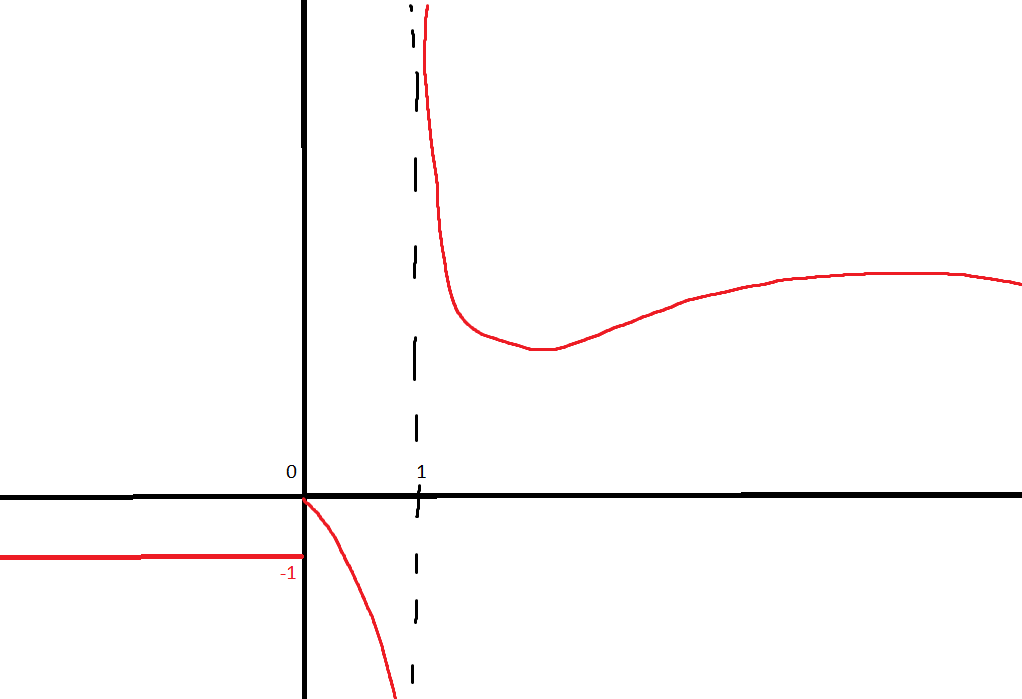
\includegraphics[width=0.8\textwidth]{image.png}\]
    \end{enumerate}


\end{enumerate}
\end{document}